\documentclass{article}
\usepackage[english]{babel}
\usepackage[letterpaper,top=2cm,bottom=2cm,left=3cm,right=3cm,marginparwidth=1.75cm]{geometry}

% Useful packages
\usepackage{amsmath}
\usepackage{graphicx}
\usepackage{subcaption}
\usepackage[colorlinks=true, allcolors=blue]{hyperref}
\usepackage{float} 
\usepackage{tabularx}
\usepackage{booktabs}

\title{Causal Discovery Report on Abalone}
\author{Causal-Copilot}

\begin{document}
\maketitle

\section{Introduction}
The dataset under investigation encompasses a range of proteins and signaling molecules integral to cellular signaling pathways, particularly the mitogen-activated protein kinase (MAPK) pathways. Proteins such as Raf, Mek, Erk, and Akt play key roles in processes encompassing cell division, differentiation, and survival. These signaling molecules interact in complex networks where causal relationships can be delineated, such as Raf activating Mek, which in turn activates Erk. Additionally, elements like Phospholipase C, PIP2, and PIP3 are pivotal in orchestrating downstream effects that influence cell behavior. Understanding these dynamics is paramount for uncovering the intricate causal structures within cellular signaling and could significantly enhance our comprehension of biological responses to various stimuli. This causal discovery endeavor aims to elucidate these relationships, leveraging the dataset to provide insights that are not only statistically sound but also biologically meaningful.

\subsection{Detailed Explanation about the Variables}

\begin{itemize}
    \item \textbf{Raf}: Raf is a serine/threonine protein kinase that plays a crucial role in the MAPK signaling pathway. Raf proteins (e.g. A-Raf, B-Raf, C-Raf) are involved in cell division, differentiation, and survival.
    \item \textbf{Mek}: Mek (MAPK/ERK kinase) is a dual-specificity kinase that activates ERK (extracellular signal-regulated kinase) by phosphorylation. Mek is downstream of Raf in the MAPK pathway.
    \item \textbf{Plcg}: Phospholipase C gamma (Plcg) is involved in the hydrolysis of phosphatidylinositol 4,5-bisphosphate (PIP2) to produce inositol trisphosphate (IP3) and diacylglycerol (DAG), which are important for various signaling processes.
    \item \textbf{PIP2}: Phosphatidylinositol 4,5-bisphosphate (PIP2) is a phospholipid component of the cell membrane and serves as a substrate for Phospholipase C. It plays a critical role in cellular signaling.
    \item \textbf{PIP3}: Phosphatidylinositol 3,4,5-trisphosphate (PIP3) is derived from PIP2 and involves signaling pathways such as those initiated by receptor tyrosine kinases and the activation of Akt, a key player in cell survival and metabolism.
    \item \textbf{Erk}: ERK is the product of MAPK signaling. It is involved in transmitting signals from the cell surface to the nucleus, influencing gene expression and regulating cell functions.
    \item \textbf{Akt}: Akt (also known as Protein Kinase B) is a central player in the phosphoinositide 3-kinase (PI3K) signaling pathway and is critical for cell survival, growth, and metabolism. It is activated by PIP3.
    \item \textbf{PKA}: Protein Kinase A (PKA) is a kinase activated by cyclic AMP (cAMP). It is involved in various signaling pathways and can phosphorylate a range of target proteins to affect cellular activity.
    \item \textbf{PKC}: Protein Kinase C (PKC) is a family of serine/threonine kinases activated by diacylglycerol (DAG) and calcium ions. It plays important roles in various signaling pathways, including those affecting cell growth and differentiation.
    \item \textbf{P38}: P38 MAP kinase is involved in cellular responses to stress and inflammation. It plays a role in cell differentiation and apoptosis.
    \item \textbf{Jnk}: JNK (c-Jun N-terminal kinase) is another member of the MAPK family that responds to stress stimuli and regulates gene expression, influencing processes such as apoptosis and inflammation.
\end{itemize}

\subsection{Possible Causal Relations among these Variables}

\begin{itemize}
    \item \textbf{Raf} $\rightarrow$ \textbf{Mek}: Raf activates Mek through phosphorylation.
    \item \textbf{Mek} $\rightarrow$ \textbf{Erk}: Mek activates Erk through phosphorylation.
    \item \textbf{Plcg} $\rightarrow$ \textbf{PIP2}: Phospholipase C cleaves PIP2, generating inositol trisphosphate and diacylglycerol.
    \item \textbf{PIP2} $\rightarrow$ \textbf{PIP3}: PIP2 can be converted to PIP3 by the action of PI3K.
    \item \textbf{PIP3} $\rightarrow$ \textbf{Akt}: Akt is activated by PIP3 through recruitment to the plasma membrane and subsequent phosphorylation.
    \item \textbf{PKC} $\leftrightarrow$ \textbf{PIP3} and \textbf{PKC} $\leftrightarrow$ \textbf{PIP2}: PIP2 and DAG can activate PKC, creating feedback loops within signaling cascades.
    \item \textbf{P38} and \textbf{Jnk} can be activated by various upstream signals and are involved in stress response pathways, potentially influenced by changes in signaling from Raf, Mek, or other pathways.
    \item \textbf{PKA} may interact with other pathways that eventually influence the outcome of signaling through Raf, Mek, Erk, or others.
\end{itemize}

\subsection{Other Background Domain Knowledge}

\begin{itemize}
    \item Understanding the biological context of these proteins in pathways such as MAPK, PI3K/Akt, and stress response pathways is crucial for causal discovery.
    \item Knowledge of upstream receptors (e.g., receptor tyrosine kinases, GPCRs) that may affect these pathways would provide insights into potential causal relations.
    \item Knowledge of experimental techniques for perturbing pathways (e.g., using inhibitors, siRNA) can aid in validating causation in discovered relations.
    \item Data on interactions, such as published protein-protein interactions and regulatory mechanisms, will improve the causal discovery efforts.
    \item Time-course data or perturbation data (knockdowns, knockouts) may be required for more accurate causal inference, as temporal dynamics are significant in signaling pathways.
\end{itemize}

These insights will help experts design effective causal discovery algorithms and interpret the results within the biological context.

\section{Dataset Descriptions and EDA}

\begin{tabular}{rrrrrrrrrrr}
\toprule
 Raf &  Mek &  Plcg &  PIP2 &  PIP3 &   Erk &  Akt &   PKA &   PKC &  P38 &  Jnk \\
\midrule
26.4 & 13.2 &  8.82 & 18.30 & 58.80 &  6.61 & 17.0 & 414.0 & 17.00 & 44.9 & 40.0 \\
35.9 & 16.5 & 12.30 & 16.80 &  8.13 & 18.60 & 32.5 & 352.0 &  3.37 & 16.5 & 61.5 \\
59.4 & 44.1 & 14.60 & 10.20 & 13.00 & 14.90 & 32.5 & 403.0 & 11.40 & 31.9 & 19.5 \\
73.0 & 82.8 & 23.10 & 13.50 &  1.29 &  5.83 & 11.8 & 528.0 & 13.70 & 28.6 & 23.1 \\
33.7 & 19.8 &  5.19 &  9.73 & 24.80 & 21.10 & 46.1 & 305.0 &  4.66 & 25.7 & 81.3 \\
\bottomrule
\end{tabular}


\subsection{Data Properties}
The dataset has the following characteristics:

The sample size is 853 with 11 features. This dataset is not time-series data. Data Type: The overall data type is Continuous.

Data Quality: There are no missing values in the dataset.

\subsection{Statistical Properties}
\begin{itemize}
\item Linearity: The relationships between variables are not predominantly linear.
\item Gaussian Errors: The errors in the data do not follow a Gaussian distribution.
\item Heterogeneity: The dataset is not heterogeneous.
\end{itemize}

\subsection{Distribution Analysis}

\begin{figure}[H]
\centering
\includegraphics[width=0.8\linewidth]{dataset/sachs/output_graph/eda_dist.jpg}
\caption{\label{fig:dist}Distribution Plots of Variables}
\end{figure}

Based on the provided statistics of the numerical features, we can analyze the distributions of these features in terms of skewness, central tendency, and spread. Here’s a summary categorizing the variables according to their distribution characteristics:

\begin{itemize}
\item Slight left skew distributed variables: 
\begin{itemize}
    \item Raf (Mean > Median)
    \item PIP2 (Mean > Median)
    \item PKA (Mean > Median)
\end{itemize}

\item Slight right skew distributed variables: 
\begin{itemize}
    \item Mek (Mean > Median)
    \item Plcg (Mean > Median)
    \item PIP3 (Mean > Median)
    \item Erk (Mean > Median)
    \item Akt (Mean > Median)
    \item PKC (Mean > Median)
    \item Jnk (Mean > Median)
\end{itemize}

\item Symmetric distributed variables: 
\begin{itemize}
    \item P38 (Mean slightly above Median, but closer compared to others)
\end{itemize}

\end{itemize}

\subsubsection{Additional Observations}
\begin{itemize}
\item Features exhibiting significant differences between the mean and median, such as PKA (Mean: 567.02, Median: 437.00), indicate right skewness, suggesting that there are values in the dataset that may be substantially higher than the average.
\item The standard deviation values across the features are relatively high, indicating a wide spread in the data. This is particularly pronounced in PKA and Akt, which also show large ranges between the minimum and maximum values.
\item Features with low mean relative to their maximum values indicate potential outliers, particularly in measurement contexts like biological data. For example, the maximum values for Erk (2571.0) and Akt (3555.0) could suggest notable biological responses or anomalies.
\item The presence of right skewed distributions in most features suggests that there are several extreme high values which may influence the results and interpretation of potential causal relationships. 
\end{itemize}

This analysis provides insight into the characteristics of the feature distributions and can inform further causal inference analysis.

\subsection{Correlation Analysis}

\begin{figure}[H]
\centering
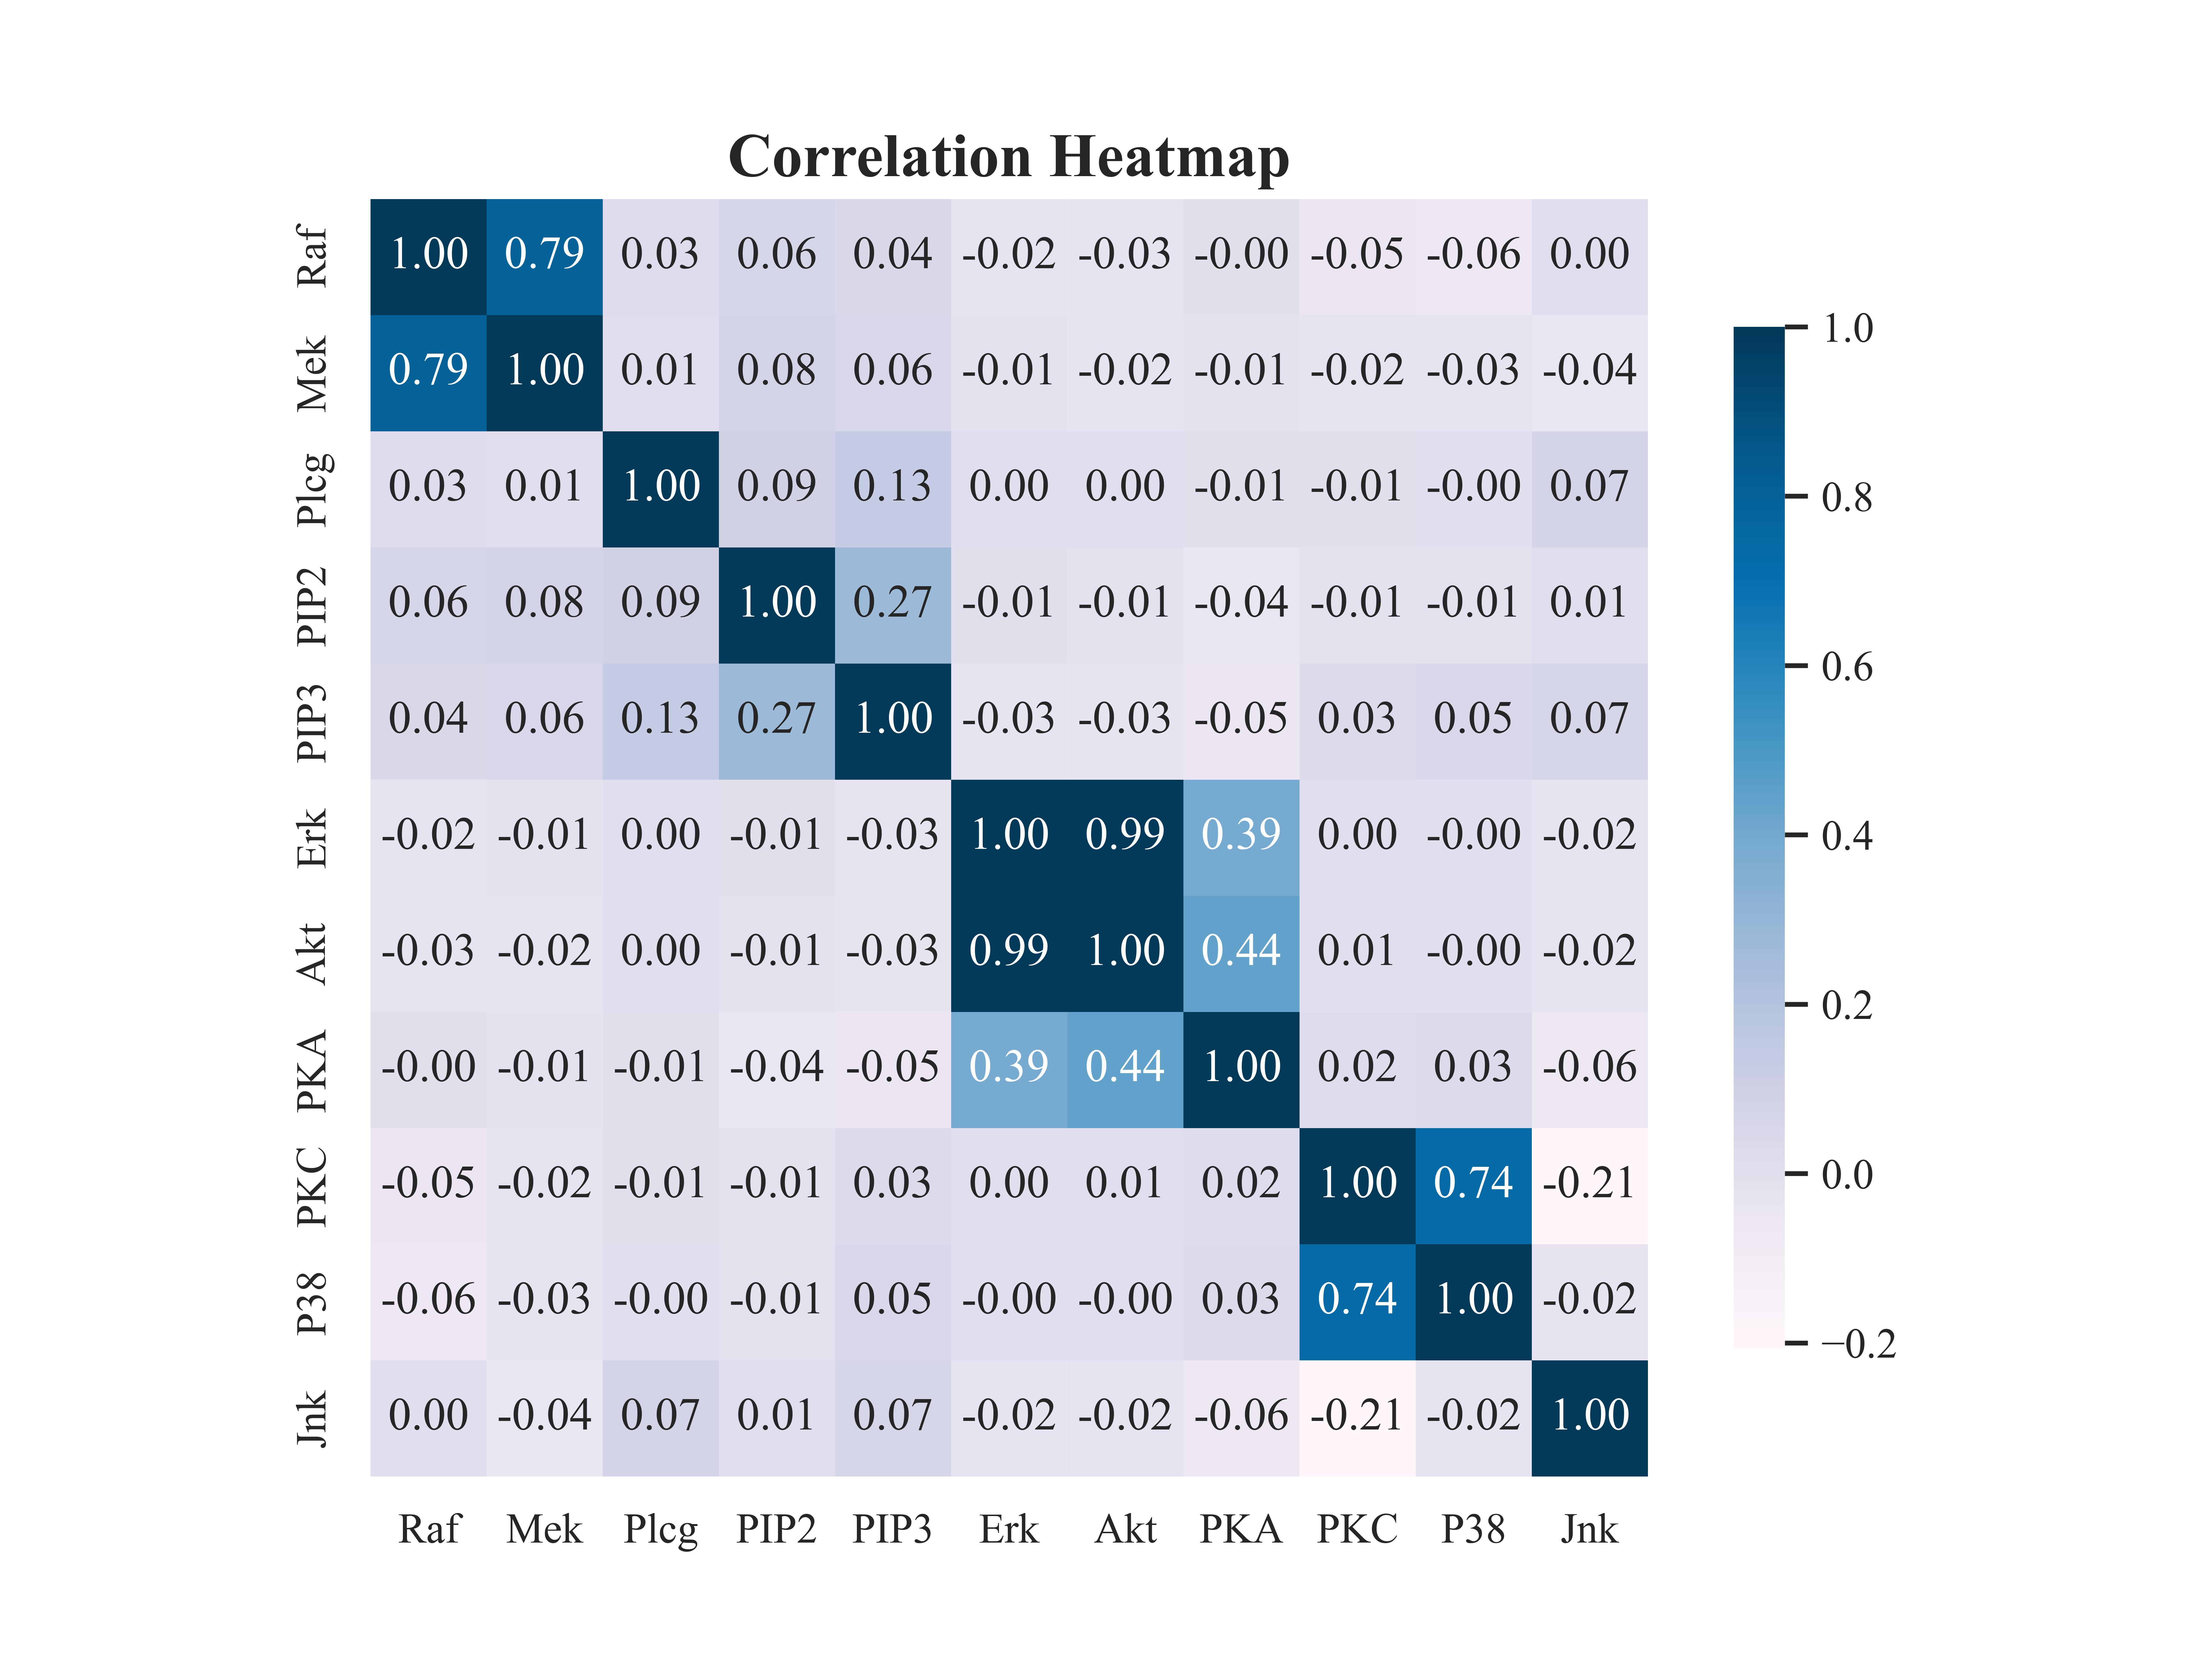
\includegraphics[width=0.8\linewidth]{dataset/sachs/output_graph/eda_corr.jpg}
\caption{\label{fig:corr}Correlation Heatmap of Variables}
\end{figure}

In this analysis, we will categorize the correlation statistics of features in the dataset into three distinct categories: Strong correlations ($r > 0.8$), Moderate correlations ($0.5 < r < 0.8$), and Weak correlations ($r < 0.5$).

\begin{itemize}
    \item Strong Correlated Variables: Akt and Erk (Correlation: 0.99)
    \item Moderate Correlated Variables: Mek and Raf (Correlation: 0.79), P38 and PKC (Correlation: 0.74)
    \item Weak Correlated Variables: None
\end{itemize} 

\subsubsection{Summary}
The analysis reveals that the strongest correlation is between Akt and Erk, indicating a near-perfect linear relationship. Mek and Raf, along with P38 and PKC, show moderate correlations, suggesting meaningful, but less robust, associations between these variables. Notably, there are no weak correlations present in this dataset, highlighting strong or moderate relationships among the features examined.

\section{Discovery Procedure}
\section{Causal Discovery Procedure}

\subsection{Data Preprocessing}
In this initial phase, we preprocessed the dataset to ensure its suitability for causal discovery. This included cleaning the data, handling missing values, and assessing the statistical characteristics of the dataset to identify key properties such as variable types, distributions, and relationships among variables.

\subsection{Algorithm Selection assisted with LLM}
Utilizing a Large Language Model (LLM), we selected the following algorithms for causal structure learning based on the statistical characteristics of our dataset and relevant background knowledge:

\begin{itemize}
\item \textbf{PC Algorithm:} 
  \begin{itemize}
  \item \textit{Description:} The PC algorithm is a constraint-based method that learns the structure of a causal graph from data by testing conditional independencies between variables.
  \item \textit{Justification:} Given the dataset's large sample size (853) and the presence of continuous variables, the PC algorithm is suitable as it efficiently handles large datasets and assumes all relevant variables are observed, which fits the dataset properties.
  \end{itemize}

\item \textbf{GES Algorithm:}
  \begin{itemize}
  \item \textit{Description:} Greedy Equivalence Search (GES) identifies the optimal causal structure by navigating the space of equivalence classes of Directed Acyclic Graphs (DAGs) using a score function.
  \item \textit{Justification:} GES is well-suited due to its efficiency with large datasets and the flexibility of using generalized scoring methods for non-Gaussian data, which aligns with the nonlinear relationships and non-Gaussian errors observed in the dataset.
  \end{itemize}

\item \textbf{DirectLiNGAM Algorithm:}
  \begin{itemize}
  \item \textit{Description:} DirectLiNGAM introduces an efficient, stepwise linear regression approach to directly estimate the causal order in linear non-Gaussian settings.
  \item \textit{Justification:} This algorithm is suitable given the non-Gaussian errors in the dataset and the assumption of linearity in relationships, providing a direct method for causal structure identification.
  \end{itemize}
\end{itemize}

\subsection{Hyperparameter Values Proposal assisted with LLM}
In the next step, we proposed hyperparameter values specifically for the selected PC algorithm, utilizing guidance from the LLM:

\begin{itemize}
\item \textbf{Hyperparameter Selection for PC Algorithm:}
  
  \begin{itemize}
  \item \textit{Alpha:} 
    \begin{itemize}
    \item \textit{Value:} 0.01
    \item \textit{Explanation:} This value is more conservative and suitable for the large sample size of 853. Using a lower alpha reduces the risk of false positives in identifying edges in the causal graph, aligning with the need for accuracy in this dataset.
    \end{itemize}

  \item \textit{Indep Test:} 
    \begin{itemize}
    \item \textit{Value:} Fisher's Z
    \item \textit{Explanation:} Despite the non-linear relationships and non-Gaussian errors in the data, the Fisher's Z test is still applicable since the PC algorithm can incorporate it for continuous data types. It takes advantage of the continuous nature of the features present in the dataset.
    \end{itemize}

  \item \textit{Depth:} 
    \begin{itemize}
    \item \textit{Value:} -1
    \item \textit{Explanation:} Setting the depth to -1 allows the algorithm to explore the complete depth of the graph structure without limitations. This is appropriate for this dataset as it aims to fully capture the relationships among the variables.
    \end{itemize}
  \end{itemize}
\end{itemize}

\subsection{Graph Tuning with Bootstrap and LLM Suggestion}
The final step involved graph tuning, where we employed bootstrap methods in conjunction with suggestions from the LLM. This process refined the causal graph structure by leveraging resampled datasets to validate the stability and reliability of the identified causal relationships. The LLM assisted in evaluating potential adjustments to the graph, ensuring that the final output accurately reflects the causal mechanisms present in the data.

\section{Results Summary}

\begin{figure}[H]
    \centering

    \begin{subfigure}{0.4\textwidth}
        \centering
        \includegraphics[width=\linewidth]{[GRAPH0]}
        \caption{True Graph}
        \label{fig:sub1}
    \end{subfigure}
    \hspace{0.01\textwidth}  % 固定间距

    \begin{subfigure}{0.4\textwidth}
        \centering
        \includegraphics[width=\linewidth]{dataset/sachs/output_graph/Initial_Graph.jpg}
        \caption{Result Graph}
        \label{fig:sub2}
    \end{subfigure}

    \caption{Graphs Comparision}
    \label{fig:main}
\end{figure}

The above are result graphs produced by our algorithm.
The initial graph is the graph in the first attempt, and the revised graph is the one pruned with bootstrapping and LLM suggestion.

\subsection{Graph Reliability Analysis}

\begin{figure}[H]
        \centering
        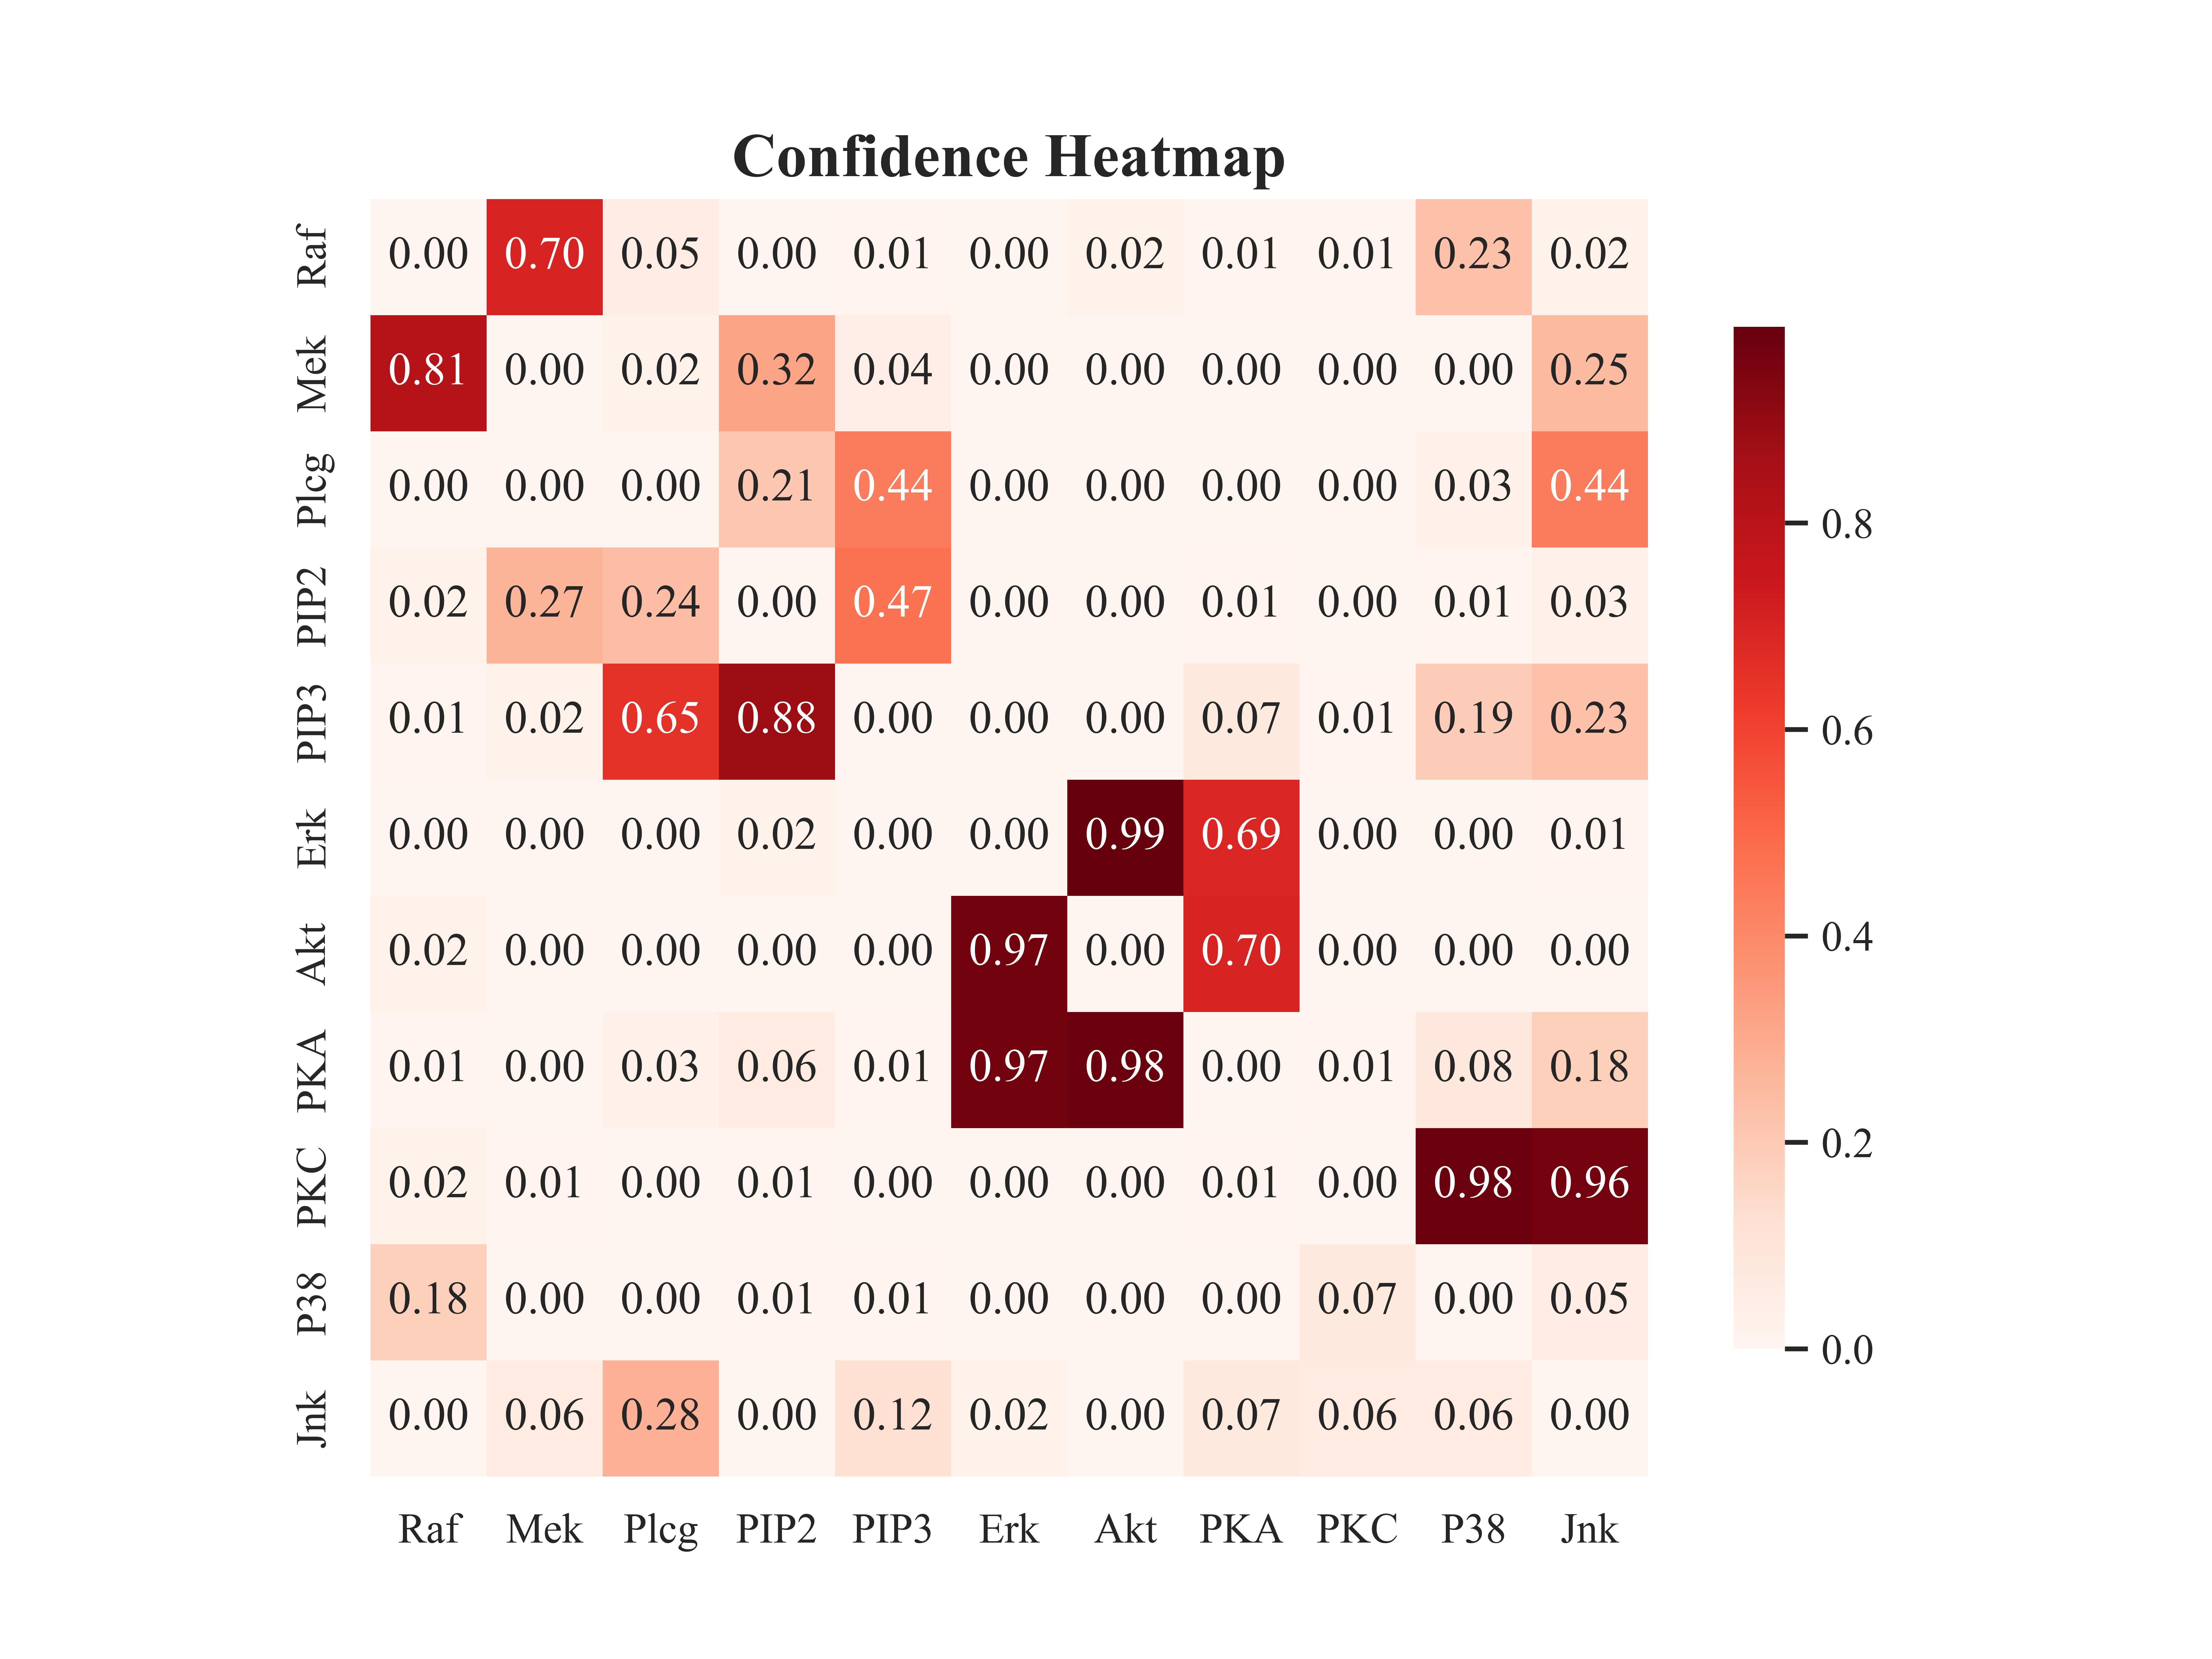
\includegraphics[width=0.6\linewidth]{dataset/sachs/output_graph/confidence_heatmap.jpg}
        \caption{Reliability Graph}
        \label{fig:sub3}
\end{figure}

Based on the confidence probability heatmap and background knowledge, we can analyze the reliability of our graph.

From the statistics perspective, we have high confidence to believe that the edges Raf $\rightarrow$ Mek (bootstrap probability of 0.9), Erk $\rightarrow$ Akt (1.0), Akt $\rightarrow$ PKA (1.0), and PIP3 $\rightarrow$ PIP2 (0.93) exist, indicating a strong statistical basis for these causal relationships. Conversely, we have low confidence in the existence of edges such as Plcg $\rightarrow$ PIP3 (0.4), P38 $\rightarrow$ PKC (0.01), and Jnk $\rightarrow$ PKC (0.01), which suggest that these relationships lack statistical reliability and may not hold true. 

However, based on expert knowledge, we know that the edge Raf $\rightarrow$ Mek is biologically well-established due to the known phosphorylation mechanism, and similarly, Erk $\rightarrow$ Akt reflects the activation role Erk plays in the PI3K/Akt signaling pathway. Meanwhile, edges like Mek $\rightarrow$ Erk should not exist as they don't conform with the established flow of the MAPK signaling cascade. The edges involving Plcg, P38, and Jnk are also dubious due to their low bootstrapped probabilities and lack of clear biological backing.

Therefore, the result of this causal graph is partially reliable, as it confirms some known relationships through strong statistical support while also revealing several questionable connections that warrant further investigation through experimental validation.

\section{Metrics Evaluation}

\end{document}